\chapter{Preliminaries} \label{Preliminaries}
%
\section{Overview}
%
\section{Hash function}
%
In this section, we will define the syntax and the security model of the cryptographic hash function, as introduced in \cite{Katz:2007:IMC:1206501}. We will slightly change their definition, because we assume no key as input to the hash function. In our case, the only input is a message.
%
\begin{definition}{(Hash function - syntax)} \textnormal{\cite{Katz:2007:IMC:1206501}}
A \textbf{hash function} is a probabilistic polynomial-time algorithm $H$
fulfilling the following:
\begin{itemize}
  \item[$\bullet$] There exists a polynomial $l$ such that $H$ is (deterministic) polynomial-time
  algorithm that takes as input any string $x \in { \{ 0,1 \}}^*$, and outputs
  a string $H(x) \in { \{ 0,1 \}}^{l(n)}$.
\end{itemize}
If for every $n$, $H$ is defined only over inputs of length $l'(n)$ and $l'(n) > l(n)$, then
we say that $H$ is a \textbf{fixed-length hash function} with length parameter $l'$. The output of a hash function is called digest.
\end{definition}

Notice that in the fixed-length case we require that $l'$ be greater than $l$. This ensures that the
function is a hash function in the classic sense in that it \textit{compresses} the input. We remark
that in the general case we have no requirement on $l$ because the function takes for input all (finite) binary strings. Thus, by definition, it also compresses.

We will now define security for this model. We begin by defining a game for a hash function $H$, an adversary $\mathcal{A}$ and a security parameter $n$:
\\

\textbf{The collision-finding game ${Hash-coll}_{\mathcal{A},H}(n)$:} \cite{Katz:2007:IMC:1206501}
\begin{enumerate}
  \item The adversary $\mathcal{A}$ outputs a pair $x$ and $x'$. \\
  Formally, $(x,x') \leftarrow \mathcal{A}(s)$.
  \item The output of the experiment is $1$ if and only if $x \neq x'$ and $H(x) = H(x')$. In such a case we say that $\mathcal{A}$ has found a collision.
\end{enumerate}
%
The definition of collision resistance for hash functions states that no efficient adversary can find a collision except with negligible probability.
%
\begin{definition} \textnormal{\cite{Katz:2007:IMC:1206501}}
  A hash function $H$ is \textbf{collision resistant} if for all probabilistic polynomial-time adversaries $\mathcal{A}$ there exists a negligible function $\textbf{negl}$ such that

\begin{equation}\label{eqn:collision}
  Pr[{Hash-coll}_{\mathcal{A},H}(n) = 1] \leq \textbf{negl} \: (n)
\end{equation}
\end{definition}
%
%%%%%%%%%%%%%%%%%%%%%%%%%%%%%%%%%%%%%%%%%%%%%%%%%%%%%%%%%%%%%%%%%%%%%%%%%%%%%%%%
%%%%%%%%%%%%%%%%%%%%%%%%%%%%%%%%%%%%%%%%%%%%%%%%%%%%%%%%%%%%%%%%%%%%%%%%%%%%%%%%
%% The next section is not at all ready. Much of the language is taken from
%% @Kostis. Remember to take the information and present it, with your own words
%% or at least give credit to what is taken from others.
%%%%%%%%%%%%%%%%%%%%%%%%%%%%%%%%%%%%%%%%%%%%%%%%%%%%%%%%%%%%%%%%%%%%%%%%%%%%%%%%
%%%%%%%%%%%%%%%%%%%%%%%%%%%%%%%%%%%%%%%%%%%%%%%%%%%%%%%%%%%%%%%%%%%%%%%%%%%%%%%%
%
\section{\label{sec:merkle-trees}Merkle Trees}
In this section we will describe a data structure needed by the meticulous reader in order to understand the description of the \hyperref[sec:Bitcoin]{Bitcoin protocol} (\hyperref[sec:Bitcoin]{section }~\ref{sec:Bitcoin}).
A Merkle tree~\cite{merkle} is a data structure which allows a party to commit to a set of items using only a single hash and prove the inclusion of any item in the committed set, by providing a logarithmic proof in terms of the cardinality of the set.

More specifically, the hashes of the items consist the leafs of the tree and the last level. The internal levels are defined recursively as follows: To create level $k-1$ each pair of level $k$ $(A, B)$ is transformed as a node of value $H(A || B)$ which points to both $A$ and $B$. If the number of nodes at level $k$ is odd, the last node at that level is paired with itself\footnote{This specific construction is the one Bitcoin implements. There are various other constructions which are beyond the scope of our work.}.

Merkle trees are useful in Bitcoin in order to commit to a set of transactions that will be included in a block while keeping the block header of a constant size.

To provide proof of inclusion, all a prover has to do is provide a path of siblings up to the root $\sf{siblings}$ and a bit vector $\sf{left}$ indicating whether each sibling is on the left or the right. The verification process is shown in \hyperref[alg:merkle-verification]{Algorithm}~\ref{alg:merkle-verification}~\cite{gtklocker}.

\begin{algorithm}
  \caption{\label{alg:merkle-verification}The \textsf{Verify} algorithm
    for a Merkle proof}
    \begin{algorithmic}[1]
      \Function{\sf Verify$_{\sf root}$}{\sf leaf, siblings, left}
            \State \sf{currentHash}$\gets$\sf{leaf}
            \While{$\sf{left} \neq []$}
              \State \sf{siblingIsLeft}$\gets$\sf{left.shift()}
              \If{\sf{siblingIsLeft}}
                \State \sf{currentHash}$\gets$\sf{H(siblings.shift() || currentHash)}
              \Else
                \State \sf{currentHash}$\gets$\sf{H(currentHash || siblings.shift())}
              \EndIf
            \EndWhile
            \State\Return{currentHash = root}
        \EndFunction
    \end{algorithmic}
\end{algorithm}

An example of a Bitcoin Merkle tree, along with a proof of inclusion for $K$ can be seen on Figure~\ref{fig:merkletree}.

\begin{figure}[ht!]
  \centering
  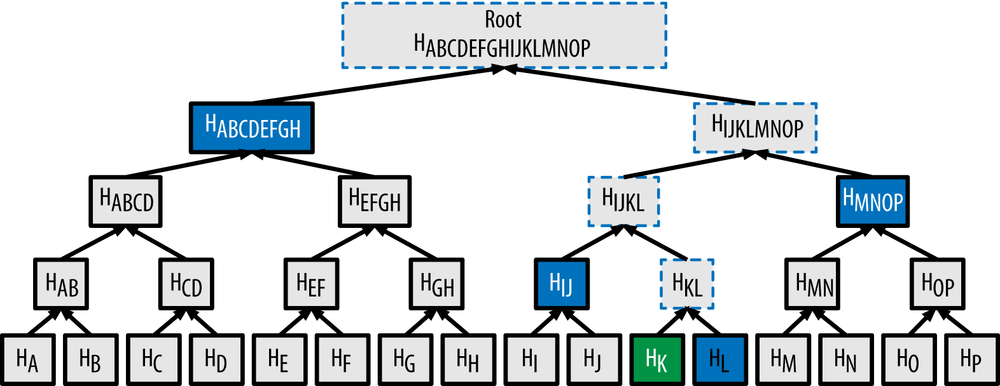
\includegraphics[width=0.9\columnwidth,keepaspectratio]{Images/merkle-tree-proof.png}
  \caption{A Bitcoin Merkle tree. Source:~\cite{mastering}}
  \label{fig:merkletree}
\end{figure}
%
\section{Password Scramblers}
Passwords\footnote{Passphrases and personal identification numbers (PINs) are considered "passwords", in this context.} are user-memorizable secrets. Typical (user-chosen) passwords often suffer from low entropy and can be attacked by trying out all possible password candidates. If we let asside the case of a dedicated cryptographic protocol on an interactive session, the next best protection are password scramblers performing "key-stretching". Christian Forler, Stefan Lucks and Jakob Wenzel~\cite{ForlerLW13}, give three basic conditions a good password scrambler should satisfy at least:

\begin{enumerate}
  \item \label{Condition 1} Given a password $pwd$, computing $PS(pwd)$ should be "fast enough" for the user.
  \item \label{Condition 2} Computing $PS(pwd)$ should be "as slow as possible", without contradicting \hyperref[Condition 1]{condition}~\ref{Condition 1}.
  \item Given $y=PS(pwd)$, there must be no significantly faster way to test $q$ password candidates $x_1, x_2, \dots, x_q$ for $PS(x_i)=y$ than by actually computing $PS(x_i)$ for each $x_i$.
\end{enumerate}
Tratidionally, most password scramblers satisfy \hyperref[Condition 2]{condition}~\ref{Condition 2} by iterating a cryptographic primitive (a block cipher or hash function) many times. However, an adversary with $b$ computing units ("cores") can try $b$ different passwords in parallel. With today's availability of graphical processing units (GPUs), slowing down these kind of attacks becomes a pressing question.
%
\section{Memory-Hard Functions}
In this section we will define the notion of the memory-hard function in the Parallel Random Oracle Model (pROM) of \cite{Alwen:2015:HPC:2746539.2746622}, as introduced in \cite{cryptoeprint:2016:875}. First, we will define the model along with the associated complexity notions.

\paragraph{The parallel Random Oracle Model.} We consider an algorithm $\mathcal{A}$ executing in the pROM of computation \cite{Alwen:2015:HPC:2746539.2746622}. Let this algorithm be repeated an arbitrary amount of times. After each invocation we make states. At invocation $i \in \{ 1,2, \dots \}$ algorithm $\mathcal{A}$ keeps the state $\sigma_{i-1}$ it produced. Next $\mathcal{A}$ can make calls $\textbf{q}_i = (q_{1,i}, q_{2,i}, \dots)$
to the \textit{fixed input length random oracle $H$} (ideal compression function). After it receives the digest of $H$, is allowed to perform arbitrary computation before producing its output (the next state $\sigma_i$). The state $\sigma_0$ contains the input to the computation and no other state is kept by $\mathcal{A}$. Now, we need some complexity notions to be defined.

The cumulative memory complexity (CMC) is defined to be
\begin{equation}
    cmc(\mathcal{A}) = \underset{H}{\mathbb{E}} \Bigg{[} \underset{x,r}{\max} \sum_{i} \lvert \sigma_i \rvert \Bigg{]}
\end{equation}
where $\lvert \sigma \rvert$ is the bit-length of state $\sigma$, the expectation is taken over the choice of $H$ and $max_{x,r}$ denotes the maximum over all inputs and coins of $\mathcal{A}$.

Moreover, the \textit{time complexity} (TC), $time(\mathcal{A})$ is the maximum running time of $\mathcal{A}$ in any execution. Similarly, the \textit{space complexity} (SC) is the largest state it ever outputs in any execution.

\paragraph{Oracle function.} Let $f$ be a function over strings depending on the choice of $H$. We consider the scenario in which we want to compute $f$ on $m \in \mathbb{N}^{+}$ arbitrary distinct inputs.
Let $\mathbb{A}_{f,m,q}$ be the set of pROM algorithms that accomplish this, making at most $q$ queries to
$H$. Then,

\begin{enumerate}[label=(\alph*)]
  \item $f$ is an oracle function \\

  \item The \textit{amortized cumulative memory complexity} (aCMC) of $f$ is defined to be
  \begin{equation}
      cmc_{m,q}(f) = \min \Bigg{\{} \frac{cmc(\mathcal{A})}{n} : \: n \in [m], \mathcal{A} \in \mathbb{A}_{f,n,q} \Bigg{\}}.
  \end{equation}
\end{enumerate}
This definition provides a good lower-bound on the \textit{amortized time complexity} of a function \cite{Alwen:2015:HPC:2746539.2746622}.

For more detailed information about the above, we refer the reader to the appendix of \cite{cryptoeprint:2016:875}. There are some technical details there that are beyond the scope of this thesis. Now we are ready to define properly the notion of the memory-hard function.

\begin{definition}{\textbf{(Memory-Hard Function).}}{\label{Memhard1}} \textnormal{\cite{cryptoeprint:2016:875}}
  Let $\{ f_{\sigma, \tau} \}_{\sigma, \tau \in \mathbb{N}^{+}}$ be a family of (oracle) functions and $\mathcal{N}$ be a sequential pROM algorithm which, on input $(\sigma, \tau, x)$, outputs $f_{\sigma, \tau}(x)$ in time at most $\tau \sigma$ using space at most $\sigma$. Then $F=\big{(} \{ f_{\sigma,\tau} \}, \mathcal{N} \big{)}$
  is an $(h,g,t)$-memory-hard function (for up to $m$ instances and $q$ queries) if it has memory-hardness at least $h$, memory-gap at most $g$ and throughput at least $t$ (all functions of $\sigma$ and $\tau$).

\begin{align*}
cmc_{m,q}(f_{\sigma, \tau})&\geq h(\sigma, \tau)           &  \frac{\mbox{space}(\mathcal{N})*\mbox{time}(\mathcal{N})}{cmc_{m,q}(f_{\sigma, \tau})} &\leq g(\sigma, \tau)             &  \frac{\mbox{space}(\mathcal{N})}{\mbox{time}(\mathcal{N})} &\geq t(\sigma, \tau)\\
\end{align*}
%
\end{definition}

The above definition, although extremely rigid, is not that intuitive. In order to describe memory requirements, we will mention another definition given in \cite{ForlerLW13}, without causing any conflict with \hyperref[Memhard1]{definition}~\ref{Memhard1}. Before we give the second definition, one should notice that for any parallelized attack, using $b$ cores, the required memory per core is decreased by a factor of $\frac{1}{b}$, and vice versa.

\begin{definition}{\textbf{(Memory-Hard Function - intuitive).}}\textnormal{\cite{ForlerLW13}}
  Let $g$ denote the memory cost factor. For all $\alpha > 0$, a memory-hard function $f$ can be computed on a Random Access Machine using \textbf{space}$(g)$ space and \textbf{time}$(g)$ operations, where \textbf{space}$(g) \in \Omega(\mbox{\textbf{time}}(g)^{1-\alpha})$.\\

  \noindent Thus, for \textbf{space}$(\cdot)$\:$\cdot$\:\textbf{time}$(\cdot)$\:$=G^2$ with $G=2^g$, using $b$ cores, we have
  \begin{equation}\label{eqn:memhard}
    \Bigg{(} \frac{1}{b} \cdot \mbox{\textbf{space}}(\cdot) \Bigg{)} \cdot \bigg{(} b \cdot \mbox{\textbf{time}}(\cdot) \bigg{)} = G^2.
  \end{equation}
\end{definition}
In their paper, a formal generalization of this notion is given, but it is beyond of the scope of this thesis. For more information about memory-hardness the reader is refered to their work~\cite{ForlerLW13}.
%
\section{Pseudorandom Functions} \label{PRF}
In cryptography, a pseudorandom function family, abbreviated $PRF$, is a collection of efficiently-computable functions which emulate a random oracle in the following way: no efficient algorithm can distinguish (with significant advantage) between a function chosen randomly from the PRF family and a random oracle (a function whose outputs are fixed completely at random). With that in mind,
we must first recall the definition of oracle indistinguishability and then proceed to define a pseudorandom function.

\begin{definition}{(Oracle Indistinguishability).} \textnormal{\cite{ACI}}
  Let $\{ O_n \}_{n \in \mathbb{N}}$ and $\{ O'_{n} \}_{n}$ be ensembles where $O_n, O'_n$ are probability
  distributions over functions $f: \{ 0,1 \}^{l_1(n)} \rightarrow \{ 0,1 \}^{l_2(n)}$ for some polynomials $l_1(\cdot)$, $l_2(\cdot)$. We say that $\{ O_{n} \}_{n}$ and $\{ O'_{n} \}_{n}$ are \textbf{computationally indistinguishable} (denoted by $\{ O'_{n} \}_{n} \approx \{ O'_n \}_{n \in \mathbb{N}}$
  ) if for all non-uniform p.p.t. oracles machines $D$, there exists a negligible function $\epsilon(\cdot)$ such that $\forall n \in \mathbb{N}$
  \begin{equation}{\label{oracle}}
    \Bigg{\lvert} \: Pr \big{[} F \leftarrow O_n : D^{F(\cdot)}(1^n)=1 \big{]} - Pr \big{[} F \leftarrow O'_n : D^{F(\cdot)}(1^n)=1 \big{]} \: \Bigg{\rvert} < \epsilon(n).
  \end{equation}
\end{definition}

\begin{definition}{(Pseudo-random Function).} \textnormal{\cite{ACI}}
  A family of functions $\big{\{} f_s: \{ 0,1 \}^{\lvert s \rvert} \rightarrow \{ 0,1 \}^{\lvert s \rvert} \big{\}}_{s \in \{ 0,1 \}^{*}}$ is \textbf{pseudo-random} if
  \begin{itemize}
    \item[$\bullet$] (Easy to compute): $f_s(x)$ can be computed by a p.p.t. algorithm that is given input $s$ and $x$
    \item[$\bullet$] (Pseudorandom): $\big{\{} s \leftarrow \{ 0,1 \}^n: f_s \big{\}}_n \approx \big{\{} F \leftarrow RF_n: F \big{\}}_n$.
  \end{itemize}
\end{definition}
Notice that if someone knows $s$ then it is easy to distinguish $f_s$ from a random function. In order to consider this function indistinguishable from a random function, one should keep seed $s$ secret.
%

\section{Pebbling game}
Hellman presented in \cite{Hellman:2006:CTT:2263346.2269686} a possibility to trade memory/space $S$ against time $T$ in attacking cryptographic algorithms, i.e. he has introduced the idea of a time-memory trade-off ($TMT$) in terms of generic attacks. Hence, we can assume that an adversary with access to this algorithm and restricted resources is always looking for a sweet spot to optimize $S \cdot T$. For, studying the $TMT$, one needs to choose a certain model. But first we must introduce the reader to the notion of the \textit{directed acyclic graph}.

\begin{definition}{(Directed Acyclic Graph).}\textnormal{\cite{ForlerLW13}}
  Let $\Pi(\mathcal{V},\mathcal{E})$ be a graph consisting of a set of vertices $\mathcal{V}=(v_0,v_1,\dots,v_{n-1})$ and a set of edges $\mathcal{E}=(e_0,e_1,\dots,e_{l-1})$, where $\mathcal{E}=\varnothing$ is a valid variant. $\Pi(\mathcal{V},\mathcal{E})$ is a \textbf{directed acyclic graph}, if every edge in $\mathcal{E}$
  consists of a starting vertex $v_i$ and an ending vertex $v_j$, with $i \neq j$. A path through $\Pi(\mathcal{V},\mathcal{E})$ beginning at vertex $v_i$ must never reach $v_i$ again (else, there would be a cycle). If there exists a path from a vertex $v_i$ to a vertex $v_j$ in the graph with $i \neq j$, we will write $v_i \leq v_j$.
\end{definition}

In 1970, Hewitt and Paterson introduced a method for analyzing $TMTs$ on directed acyclic graphs ($DAG$), called \textit{pebble game}. It has been occasionally used in cryptographic context, see, e.g. \cite{Dziembowski:2011:KSR:2033036.2033061} for a recent example. The pebble game model is restricted to $DAGs$ with bounded in-degree and can be seen as a single-player game.

\begin{definition}{(Parallel/Sequential Graph Pebbling).}\textnormal{\cite{cryptoeprint:2016:875}}
  Let $G=(\mathcal{V},\mathcal{E})$ be a $DAG$ and let $T \subseteq \mathcal{V}$ be a target set of nodes to be pebbled. A pebbling configuration (of $G$) is a subset $P_i \subseteq \mathcal{V}$. A legal parallel pebbling of $T$ is a sequence $P=(P_0,\dots,P_t)$ of pebbling configurations of $G$ where $P_0 = \varnothing$ and which satisfies \hyperref[pebble:condition_1]{conditions}~\ref{pebble:condition_1}
  \hyperref[pebble:condition_2]{\&}~\ref{pebble:condition_2} below. A sequential pebbling additionally must satisfy \hyperref[pebble:condition_3]{condition}~\ref{pebble:condition_3}.

  \begin{enumerate}
    \item \label{pebble:condition_1} At some step every target node is pebbled (though not necessarily simultaneously).
%
    \begin{equation}\label{eqn:pebcondition_1}
      \forall x \in T \ \ \exists z \leq t \quad : \quad x \in P_z.
    \end{equation}
%
    \item \label{pebble:condition_2} Pebbles are added only when their predecessors already have a pebble at the end of the previous step.
%
    \begin{equation}\label{eqn:pebcondition_2}
      \forall i \in [t] \quad : \quad x \in (P_i \setminus P_{i-1}) \ \Rightarrow \ \mbox{\textbf{parents}}(x) \subseteq P_{i-1}.
    \end{equation}
%
    \item \label{pebble:condition_3} At most one pebble placed per step.
%
    \begin{equation}\label{eqn:pebcondition_3}
      \forall i \in [t] \quad : \quad \lvert P_i \setminus P_{i-1} \rvert \leq 1.
    \end{equation}
%
  \end{enumerate}
%
  We denote with $\mathcal{P}_{G,T}$ and $\mathcal{P}_{G,T}^{||}$ the set of all legal sequential and parallel pebblings of $G$ with target set $T$, respectively.
  Note that $\mathcal{P}_{G,T} \subseteq \mathcal{P}_{G,T}^{||}$. In the case where $T=\mbox{\textbf{sinks}}(G)$, we will simply write $\mathcal{P}_{G}$ and
  $\mathcal{P}_{G}^{||}$.
%
\end{definition}
%
\begin{definition}{(Time/Space/Cumulative Pebbling Complexity).}\textnormal{\cite{cryptoeprint:2016:875}}
  The time, space, space-time and cumulative complexity of a pebbling $P=\{ P_0,\dots,P_t \} \in \mathcal{P}_{G}^{||}$ are defined to be:

  \begin{align*}
    \Pi_t(P)&= t  &  \Pi_s(P)&= \underset{i \in [t]}{\max} \lvert P_i \rvert &  \Pi_{st}(P)&= \Pi_t(P) \cdot \Pi_s(P) & \Pi_{cc}(P)&= \underset{i \in [t]}{\sum} \lvert P_i \rvert .\\
  \end{align*}
  For $\alpha \in \{ s,t,st,cc \}$ and a target set $T \subseteq \mathcal{V}$, the sequential and parallel pebbling complexities of $G$ are defined as

  \begin{align*}
    \Pi_\alpha(G,T)&= \underset{P \in \mathcal{P}_{G,T}}{\min} \Pi_{\alpha}(P) &  &\mbox{and} & \Pi_{\alpha}^{||}(G,T)&= \underset{P \in \mathcal{P}_{G,T}^{||}}{\min} \Pi_{\alpha}(P) .\\
  \end{align*}
  When $T=\mbox{\textbf{sinks}}(G)$ we simplify notation and write $\Pi_{\alpha}(G)$ and $\Pi_{\alpha}^{||}(G)$.
%
\end{definition}
We notice that the definition comes along with the intuition about these complexities. For $\alpha \in \{ s,t,st,cc \}$ and any $G$, the parallel pebbling complexity is at most as high as the sequential,
i.e., $\Pi_\alpha(G) \geq \Pi_{\alpha}^{||}(G)$, and cumulative complexity is at most as high as space-time complexity, i.e., $\Pi_{st}(G) \geq \Pi_{cc}(G)$ and $\Pi_{st}^{||}(G) \geq \Pi_{cc}^{||}(G)$.\\

\noindent With this last definition, this chapter is concluded and all the tools needed for our analysis have been formally defined.
%
%% Information about pebbling algorithms and complexity
